\documentclass{article}
\usepackage[margin=1.0in]{geometry}
\usepackage{amssymb,amsmath,amsthm,amsfonts}
\usepackage{enumitem}
\usepackage{xcolor}
\usepackage{mathtools}
\usepackage[pdftex]{graphicx}
\graphicspath{{./images/}}

\newcommand{\Z}{\mathbf{Z}}
\newcommand{\N}{\mathbf{N}}
\newcommand{\R}{\mathbf{R}}
\newcommand{\Q}{\mathbf{Q}}
\newcommand{\C}{\mathbf{C}}

\newcommand{\id}{\mathrm{id}}
\newcommand{\op}{\mathrm{op}}
\newcommand{\diam}{\mathrm{diam}}
\newcommand{\Tr}{\mathrm{Tr}}
\newcommand{\im}{\mathrm{im}}
\newcommand{\rank}{\mathrm{rank}}

\newcommand{\cl}[1]{\overline{#1}}

\swapnumbers % places numbers before thm names

\theoremstyle{plain} % The "plain" style italicizes all body text.
	\newtheorem{thm}{Theorem}
		\numberwithin{thm}{section} % Theorem numbers are determined by section.
	\newtheorem{lemma}[thm]{Lemma}
	\newtheorem{prop}[thm]{Proposition}
	\newtheorem{cor}[thm]{Corollary}

\theoremstyle{definition}
    \newtheorem{defn}[thm]{Definition}
	\newtheorem{example}[thm]{Example}
	\newtheorem{exercise}[thm]{Exercise} %Exercise

\begin{document}
    \section{Week 2 Homework}
    \begin{exercise}
        \begin{enumerate}[label=(\alph*)]
            \item Prove that there exists an infinitely differentiable function $\alpha:\R\rightarrow \R$ such that $\alpha(t)=0$ for all $t\leq 0$, and $\alpha(t)>0$ for all $t>0$.
    
            \begin{proof}
                We define \(\alpha (t) =
                \begin{dcases}
                    0, &\text{ if } t \leq 0 ;\\
                    e^{-\frac{1}{t}} , &\text{ if } t > 0.\\
                \end{dcases}\) 
                
                Trivially \(\alpha (t) = 0 \text{ if } t \leq 0\) and \(\alpha (t) > 0 \text{ if }t > 0\). It remains to show that \(\alpha \) is infinitely differentiable.

                Since \(0\) is infinitely differentiable, and \(e^{-\frac{1}{x}}\) is infinitely differentiable for \(x > 0\), it suffices to show that derivatives of all orders of \(\alpha \) are continuous at \(t = 0\).

                We will continue by proving a lemma.

                \textbf{Lemma.} \(\forall n \in \mathbb{N}, \text{ for } t > 0 \text{, } \alpha^{(n)} (t) = Q(t)\alpha (t)\), where \(Q(x)\) is a linear combination of nonpositive integer powers of \(t\).

                We will show this using induction.
                \begin{proof}
                    When \(n=1\), fixing \(t > 0\), we have
                    \[
                        \alpha ^\prime(t) = \frac{1}{t^2}e^\frac{-1}{t} = \frac{1}{t^2}\alpha (t)
                    \]
                    We let \(Q(t) = t^{-2}\) and we are done.

                    Now suppose that the lemma holds for all \(i \leq k\), for some \(k \in \mathbb{N}\).

                    Then for \(t > 0\),
                    \[
                        \alpha ^{(k)}(t) = P(t)\alpha (t). \text{ where } P(t) \text{ is a linear combination of nonpositive integer powers of t}
                    \]
                    Taking the derivative of both sides with respect to \(t\), we obtain
                    \[
                        \alpha ^{(k+1)}(t) = P^\prime(t)\alpha (t) + P(t)\alpha ^\prime (t)
                    \]
                    The lemma holds for \(i = 1\), therefore for some \(R(t)\),
                    \[
                        P^\prime(t)\alpha (t) + P(t)\alpha ^\prime (t) = P^\prime(t)\alpha (t) + P(t)R(t)\alpha (t) = (P^\prime(t) + P(t)R(t))\alpha (t)
                    \]
                    \(P^\prime(t) + P(t)R(t)\) is a linear conbination of nonpositive integer powers of \(t\), therefore letting \(Q(t) = P^\prime(t) + P(t)R(t)\), we get our desired conclusion.

                    By the principle of induction, the lemma holds true for all \(n \in \mathbb{N}\).

                \end{proof}

                We now continue in proving that derivatives of all orders of \(\alpha\) are continuous at 0. We show this by proving that
                \[
                    \lim_{t \to 0} \alpha ^{(n)}(t) = 0 \text{, where } n \in \mathbb{N}
                \]
                We will only worry about the right hand limit, as the left hand limit always evaluates to \(0\).

                Let \(n \in \mathbb{N}\). Since we only deal with positive \(t\), by our lemma,
                \[
                    \alpha ^{(n)}(t) = Q(t)\alpha (t)
                \]
                Where \(Q(t)\) is a linear combination of nonpositive integer powers of \(t\). So
                \[
                    \lim_{t \to 0^+} \alpha ^{(n)}(t) = \lim_{t \to 0^+} Q(t)\alpha (t) = \lim_{t \to 0^+} \sum_{i=0}^k a_i t^{-i} \alpha (t)
                \]
                Where \(a_i\) are real constants and \(k \in \mathbb{N}\).

                Consider an arbitrary term \(a_i t^{-i} \alpha (t) = a_i t^{-i} e^\frac{-1}{t}\). We want to show that \(\lim_{t \to 0^+}a_i t^{-i} e^\frac{-1}{t}\) exists and is equal to 0.

                First, we will perform the substitution \(x = \frac{1}{t}\). Then the limit becomes
                \[
                    \lim_{x \to \infty} a_i x^i e^{-x} = 0
                \]
                The proof for this fact is omitted, but applying L'Hopital's rule \(i\) times produces the same result. Thus,
                \[
                    \lim_{t \to 0^+} \alpha ^{(n)}(t) = \lim_{t \to 0^+} \sum_{i=0}^k a_i t^{-i} \alpha (t) = \sum_{i=0} ^k \lim_{t \to 0^+} a_i t^{-i} \alpha (t) = \sum_{i=0} ^k 0 = 0
                \]
                Thus \(\alpha \) is infinitely differentiable everywhere.

            \end{proof}
    
            \item Prove that there exists an infinitely differentiable function $\beta:\R\rightarrow \R$ such that $\beta(t)=1$ for all $t\geq 1$, and $\beta(t)=0$ for all $t\leq 0$.
    
            \begin{proof}
                Define
                \[
                    \beta (t) = \frac{\alpha (t)}{\alpha (t) + \alpha (1-t)}
                \] 
                If \(t\geq 1\), we also have \(1-t \leq 0\). Then
                \[
                    \beta (t) = \frac{\alpha (t)}{\alpha (t)} = 1
                \]
                As well, if \(t \leq 0\), we have
                \[
                    \beta (t) = 0
                \]

                Since \(\alpha(t)\) is infinitely differentiable and \(\beta\) is composed of \(\alpha \), it follows that \(\beta\) is also infinitely differentiable.

            \end{proof}
    
            \item Prove that there exists an infinitely differentiable function $\varphi:\R\rightarrow \R$ such that $\varphi(t)=1$ for all $t\in [2,3]$, and $\varphi(t)=0$ for $t\in \R\setminus (1,4)$.
    
            \begin{proof}
                Define \(\phi (t) = \beta (t-1) \beta (4-t)\).
                Since \(\beta\) is infinitely differentiable, \(\phi\) is as well. For \(t \in [2,3]\), \(t-1 \geq 1\) and \(4-t \geq 1\). Thus
                \[
                    \phi (t) = \beta(t-1) \beta (4-t) = 1
                \]
                If \(t \in \mathbb{R} \setminus (1,4)\), then \(t-1 \leq 0\) or \(4-t \leq 0\). In each case \(\beta(t-1) = 0\) or \(\beta (4-t) = 0\), respectively, thus we have
                \[
                    \phi (t) = \beta (t-1) \beta (4-t) = 0
                \]

            \end{proof}
        \end{enumerate}
    \end{exercise}
    \pagebreak
    \begin{exercise}
        Let $S\subseteq \R^n$. Consider the following three statements:
        \begin{itemize}
            \item $S$ is a bounded subset of $(\R^n,\|\cdot\|_1)$.
            \item $S$ is a bounded subset of $(\R^n,\|\cdot\|_2)$.
            \item $S$ is a bounded subset of $(\R^n,\|\cdot\|_{\max})$.
        \end{itemize}
        Among these statements, determine which implications are true and which are false. There are six implications to investigate. Supply proof or counterexample as appropriate. Include pictures.
        \\\\
        \noindent\textbf{\textcolor{red}{Note.}} My previous submission did not consider when \(d(x,y) = 0\) when proving symmetry. As well, I made a typo when writing the max-norm. Finally, the last paragraph was not written out mathematically. This resubmission should fix those issues.
    
        \noindent\textbf{Changelog.}
        \begin{enumerate}
            \item Added an argument when proving symmetry to address division by 0
            \item Fixed max-norm typo
            \item Rewrote last explanation in a more mathematical fashion
        \end{enumerate}

        \noindent\textbf{Claim.} Each statement implies all the other statements.
        \begin{proof}
            \textbf{Lemma.} Strong equivalence is an equivalence relation.
            \begin{proof}
                Let \(d_1, d_2, d_3\) be metrics on some set \(X\). We proceed by proving each property of equivalence relations.
                \begin{enumerate}
                    \item Reflexivity:
                    Let \(\alpha = \beta = 1\). Clearly \(d_1(x,y) \leq d_1(x,y) \leq d_1(x,y)\). Thus the relation is reflexive.

                    \item Symmetry:
                    Suppose \(\hat{\alpha} d_1(x,y) \leq d_2(x,y) \leq \hat{\beta} d_1(x,y)\). Let \(\alpha = \frac{1}{\hat{\beta}}, \beta = \frac{1}{\hat{\alpha}}\). \textcolor{red}{If \(x=y\), then \(d_1(x,y) = d_2(x,y) = 0\), so the inequality trivially holds.} \textcolor{red}{Otherwise, \(d_1(x,y) > 0, d_2(x,y) > 0\)}, so we see that
                    \[
                        \hat{\alpha} \leq \frac{d_2(x,y)}{d_1(x,y)} \leq \hat{\beta} \implies \frac{1}{\hat{\beta}} \leq \frac{d_1(x,y)}{d_2(x,y)} \leq \frac{1}{\hat{\alpha}} \implies \alpha d_2(x,y) \leq d_1(x,y) \leq \beta d_2(x,y)
                    \]
                    Thus the relation is symmetric.

                    \item Transitivity:
                    Suppose that \(\hat{\alpha} d_1(x,y) \leq d_2(x,y) \leq \hat{\beta} d_1(x,y)\) and \(\tilde{\alpha} d_2(x,y) \leq d_3(x,y) \leq \tilde{\beta} d_2(x,y)\). Let \(\alpha = \hat{\alpha}\tilde{\alpha}, \beta = \hat{\beta}\tilde{\beta}\). We have
                    \[
                        \alpha d_1(x,y) = \hat{\alpha}\tilde{\alpha} \leq \tilde{\alpha}d_2(x,y) \leq d_3(x,y) \leq \tilde{\beta}d_2(x,y) \leq \hat{\beta}\tilde{\beta}d_1(x,y) = \beta d_1(x,y)
                    \]
                    \[
                        \implies \alpha d_1(x,y) \leq d_3(x,y) \leq \beta d_1(x,y)
                    \]
                    Thus the relation is transitive.
                \end{enumerate}
                Therefore, the relation is an equivalence relation.
            \end{proof}
            
            We want to show that \(\|\cdot\|_1, \|\cdot\|_2, \|\cdot\|_{\max}\) are strongly equivalent to each other. First, we will show that \(\|\cdot\|_1 \sim \|\cdot\|_{\max}\) and \(\|\cdot\|_2 \sim \|\cdot\|_{\max}\). We have that
            \[
                \frac{1}{n} \sqrt{\sum_{i=1}^n |x_i - y_i|} \leq \frac{1}{n} \sum_{i=1}^n |x_i - y_i| \leq \max _{1\leq i\leq n} \{\textcolor{red}{|x_i - y_i|}\} \leq \sqrt{\sum_{i=1}^n |x_i - y_i|} \leq \sum_{i=1}^n |x_i - y_i|
            \]
            From this, we have the inequalities
            \[
                \frac{1}{n} \sqrt{\sum_{i=1}^n |x_i - y_i|} \leq \max _{1\leq i\leq n} \{\textcolor{red}{|x_i - y_i|}\} \leq \sqrt{\sum_{i=1}^n |x_i - y_i|} \text{ and } \frac{1}{n} \sum_{i=1}^n |x_i - y_i| \leq \max _{1\leq i\leq n} \{\textcolor{red}{|x_i - y_i|}\} \leq \sum_{i=1}^n |x_i - y_i|
            \]
            \[
                \implies \frac{1}{n} \|x - y\|_2 \leq \|x - y\|_{\max} \leq \|x - y\|_2 \text{ and } \frac{1}{n} \|x - y\|_1 \leq \|x - y\|_{\max} \leq \|x - y\|_1
            \]
            \[
                \implies \|\cdot\|_2 \sim \|\cdot\|_{\max} \text{ and } \|\cdot\|_1 \sim \|\cdot\|_{\max}
            \]
            Using transitivity and symmetry we can also conclude that \(\|\cdot\|_1 \sim \|\cdot\|_2\). Thus every metric is strongly equivalent to one another. \textcolor{red}{It follows that for any \(i,j \in \{1, 2, \max\}\), there exists \(c_{ij} > 0\) such that for all \(x,y \in \mathbb{R}^n\), \(d_i(x,y) \leq c_{ij} \cdot d_j(x,y)\), meaning that for \(S \subseteq \mathbb{R}^n\), if \(S\) is bounded with respect to the 1-norm, 2-norm, or the max-norm, it is bounded with respect to the other norms as well,} from which our claim follows immediately after.

            \textbf{Pictures.}

            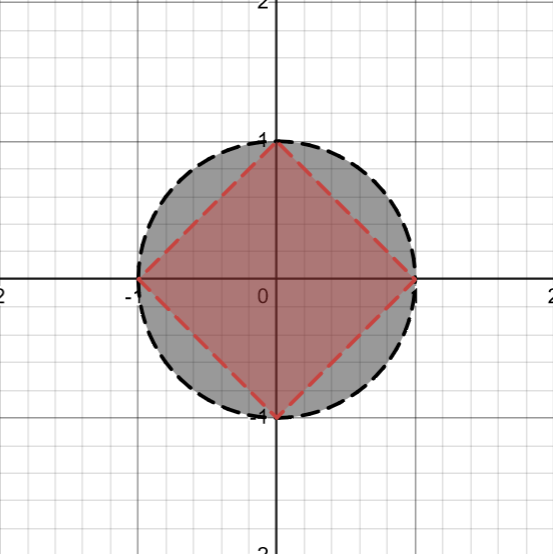
\includegraphics[width=5cm, height=5cm]{12.png}
            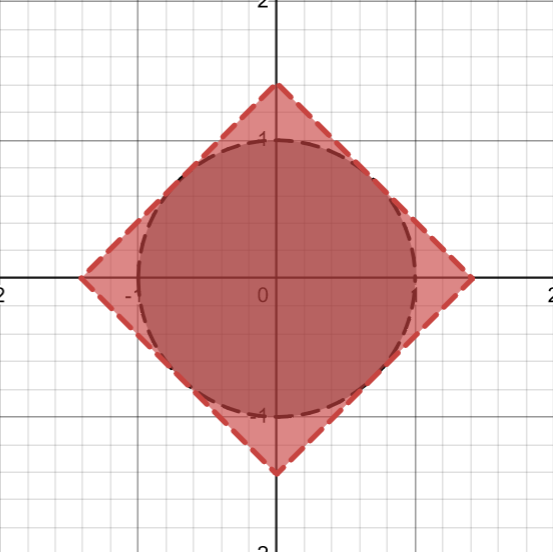
\includegraphics[width=5cm, height=5cm]{21.png}
            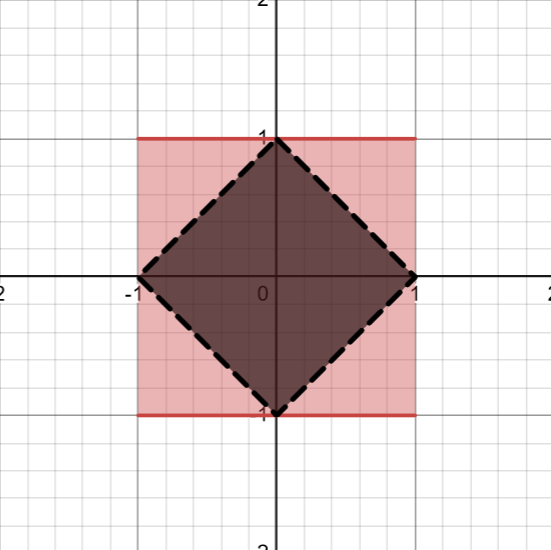
\includegraphics[width=5cm, height=5cm]{13.png}

            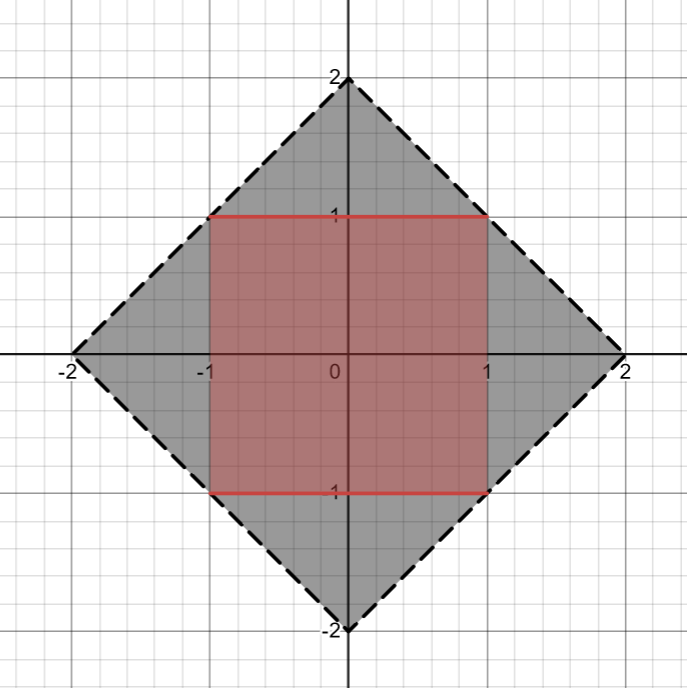
\includegraphics[width=5cm, height=5cm]{31.png}
            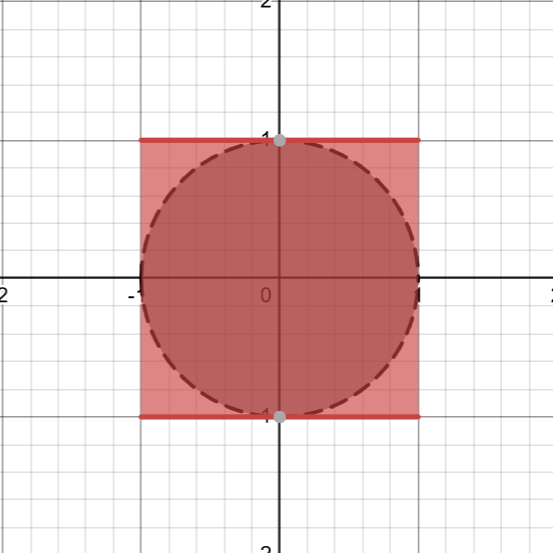
\includegraphics[width=5cm, height=5cm]{23.png}
            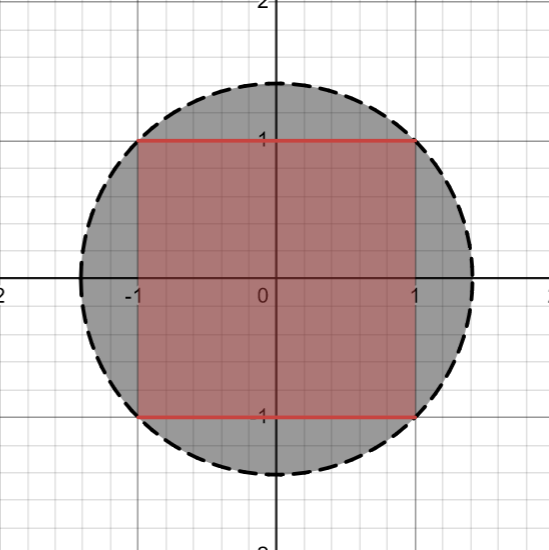
\includegraphics[width=5cm, height=5cm]{32.png}

        \end{proof}
    \end{exercise}
    \pagebreak
    \begin{exercise}
        Let $(X,\|\cdot\|_X)$ and $(Y,\|\cdot\|_Y)$ be two normed vector spaces. A linear mapping $T:X\rightarrow Y$ is called \textbf{bounded} if there exists a constant $M\geq 0$ such that
        \[ \|T(x)\|_Y \leq M \|x\|_X \quad \text{for all $x\in X$.}  \]
        Let $B(X,Y)$ denote the set of these bounded linear operators. The \textbf{operator norm} on $B(X,Y)$, denoted by $\|\cdot\|_{\mathrm{op}}$, is defined as follows:
            \[ \|T\|_{\mathrm{op}} = \sup\{ \|T(x)\|_Y : x\in X \text{ and } \|x\|_X\leq 1 \}. \]
        \begin{enumerate}[label=(\alph*)]
            \item Prove that $B(X,Y)$ is a linear subspace of $L(X,Y)$.
            
            \begin{proof}
                The 0-transformation \(\left\lVert Z(x) \right\rVert  = 0 \leq \left\lVert x \right\rVert _X \text{, } \forall x \in X\), because of the definition of a norm. Thus \(0 \in B(X,Y)\).
                Let \(T, U \in B(X,Y) \text{, } c \in \mathbb{R}\). Then for all \(x \in X\), there exist \(M, N \geq 0\) such that
                \[
                    T(x) \leq M \left\lVert x \right\rVert _X \text{ and } U(x) \leq N \left\lVert x \right\rVert _X \implies T(x) + U(x) \leq (M+N) \left\lVert x \right\rVert _X
                \] 
                Which implies that \(T+U\) is a member of \(B(X,Y)\). As well, from the first inequality, depending on if \(c \) is positive or negative, we have
                \[
                    T(x) \leq M \left\lVert x \right\rVert _X \implies cT(x) \leq  cM \left\lVert x \right\rVert _X \text{ or } -cT(x) \leq  -cM \left\lVert x \right\rVert
                \]
                Note that if \(c=0\), \(cT = 0\). Regardless, this implies that \(cT\) is a member of \(B(X,Y)\).

                Since \(0 \in B(X,Y)\)and \(B(X,Y)\) is closed under addition and scalar multiplication, \(B(X,Y)\) is a subspace of \(L(X,Y)\).

            \end{proof}
            \item Prove that $\|\cdot\|_{\mathrm{op}}$ is a norm on $B(X,Y)$.
        
            \begin{proof}
                To prove that the operator norm is a norm, we first verify that \(\left\lVert T \right\rVert _{op} = 0 \iff T = 0\).

                We denote the set of elements \(x\) in \(X\) such that \(\left\lVert x \right\rVert _X \leq 1\) as \(X^\prime\).

                Fix \(T \in B(X,Y)\) and suppose that \(T = 0\). Then for all \(x \in X^\prime \text{, } \left\lVert T(x) \right\rVert _Y = \left\lVert 0 \right\rVert _Y = 0\). Thus \(\left\lVert T \right\rVert _{op} = 0\).  
                
                Now suppose the converse, that \(\left\lVert T \right\rVert _{op} = 0\). Then 
                \[
                    \forall x \in X^\prime, \left\lVert T(x) \right\rVert _Y \leq \left\lVert T \right\rVert _{op} = 0.
                \]
                But by the definition of the norm in Y,
                \[
                    0 \leq \left\lVert T(x) \right\rVert _Y
                \]
                It follows that \(\left\lVert T(x) \right\rVert  = 0 \implies T(x) = 0\).

                To show nonnegativity, we note that for \(x \in X^\prime\),
                \[
                    \left\lVert T \right\rVert _{op} \geq \left\lVert T(x) \right\rVert _Y \geq 0
                \]

                To show homogeity, let \(T \in G(X,Y), c \in \mathbb{R}\). Then
                \[
                    \left\lVert cT \right\rVert _{op} = \sup \{ \left\lVert cT(x) \right\rVert _Y : x \in X^\prime\} = \sup \{ |c|\left\lVert T(x) \right\rVert _Y : x \in X^\prime\} = |c|\sup \{ \left\lVert T(x) \right\rVert _Y : x \in X^\prime\} = |c| \left\lVert T \right\rVert _{op}
                \] 

                Now we show that the triangle inequality holds with respect to the operator norm.

                Fix \(T, U \in B(X,Y)\). Let \(x \in X^\prime\). By definition,
                \[
                    T(x) \leq \sup T(X^\prime) \text{ and } U(x) \leq \sup U(X^\prime)
                \]
                Adding both together obtains
                \[
                    T(x) + U(x) \leq \sup T(X^\prime) + \sup U(X^\prime)
                \]
                We see that \(\sup T(X^\prime) + \sup U(X^\prime)\) is an upper bound for \(T(x) + U(x)\). By the definition of the least upper bound,
                \[
                    \sup \{T(X^\prime)+U(X^\prime)\} \leq  \sup T(X^\prime) + \sup U(X^\prime) \implies \left\lVert T+U \right\rVert _{op} \leq \left\lVert T \right\rVert _{op} + \left\lVert U \right\rVert _{op}
                \]
                Thus the operator norm is, indeed, a norm.

            \end{proof}
            \item Let $T:\R^2\rightarrow \R^2$ be the linear mapping given by $T(x,y)=(x+y,x)$. Find, with proof, the exact value of $\|T\|_{\mathrm{op}}$. (Here, $\R^2$ is equipped with the usual norm.)
            
            \textbf{Claim.} \(\left\lVert T \right\rVert _{op} = \sqrt{\frac{3+\sqrt{5}}{2}} \)

            \begin{proof}
                We will show that \(\|T(x,y)\| _2\) is bounded above by this value, and that equality is possible.
                
                Let \((x,y) \in \mathbb{R} ^2\) such that \(\sqrt{x^2 + y^2} \leq 1 \implies y \leq \pm \sqrt{1-x^2} \leq \sqrt{1-x^2}\).
                For such \((x,y)\),
                \[
                    \left\lVert T(x,y) \right\rVert _2 = \left\lVert (x+y, x) \right\rVert _2 = \sqrt{(x+y)^2 + x^2} = \sqrt{2x^2 + 2xy + y^2} 
                \]
                By the monotonicity of the squareroot,
                \[
                    \sqrt{2x^2 + 2xy + y^2} \leq \sqrt{x^2 + 2x\sqrt{1-x^2} + 1}
                \]
                We attempt to maximize this function for \(x \in [0,1]\) (The interval is the set of all \(x\) that satisfy the constraint \(x^2 + y^2 \leq 1\)). Maximizing this function is synonymous to maximizing \(f(x) = x^2 + 2x\sqrt{1-x^2} + 1\) on the interval \([0,1]\). Taking the derivative, we get
                \[
                    f^\prime(x) = 2x + 2\sqrt{1-x^2} -\frac{2x^2}{\sqrt{1-x^2}} = \frac{2x\sqrt{1-x^2} + 2 - 4x^2}{\sqrt{1-x^2}}
                \]
                Now, we find every critical point. When \(f^\prime\) is undefined, \(x = 1\).
                Now, let \(f^\prime(x) = 0\), \(x\neq 1\) . Then through a series of calculations I really don't want to type out,
                \[
                    \frac{2x\sqrt{1-x^2} + 2 - 4x^2}{\sqrt{1-x^2}} = 0 \implies 5x^4 - 5x^2 + 1 = 0 \implies x^2 = \frac{1}{2}\pm\frac{1}{2\sqrt{5}} \implies x = \sqrt{\frac{1}{2}\pm\frac{1}{2\sqrt{5}}} 
                \]
                We disregard the negative solution since we want \(x \in [0,1]\).
                Now we evaluate \(f\) at the endpoints, as well as at every point we found:
                \[
                    f(0) = 1
                \]
                \[
                    f(1) = 2
                \]
                \[
                    f\left(\sqrt{\frac{1}{2}+\frac{1}{2\sqrt{5}}}\right) = \frac{3+\sqrt{5}}{2}
                \]
                \[
                    f\left(\sqrt{\frac{1}{2}-\frac{1}{2\sqrt{5}}}\right) = \frac{3}{2}+\frac{3}{2\sqrt{5}}
                \]
                It is not too hard to see that \(f\) acheives the maximum at \(x = \sqrt{\frac{1}{2}+\frac{1}{2\sqrt{5}}}\). Then \(\sqrt{x^2 + 2x\sqrt{1-x^2} + 1}\) also acheives a maximum at \(x = \sqrt{\frac{1}{2}+\frac{1}{2\sqrt{5}}}\), which is \(\sqrt{\frac{3+\sqrt{5}}{2}}\).

                In summary, we have for all \((x,y) \in \mathbb{R} ^2\),
                \[
                    \left\lVert T(x,y) \right\rVert _2 \leq \sqrt{\frac{3+\sqrt{5}}{2}}
                \]
                Thus \(\sqrt{\frac{3+\sqrt{5}}{2}}\) is an upper bound for \(\left\lVert T(x,y) \right\rVert _2\).

                To show that \(\sqrt{\frac{3+\sqrt{5}}{2}}\) is the least upper bound, it suffices to show that \(\left\lVert T(x,y) \right\rVert _2\) can acheive that value. Indeed, if we let \(x=\sqrt{\left(\frac{1}{2}+\frac{1}{2\sqrt{5}}\right)},y= \sqrt{\left(\frac{1}{2}-\frac{1}{2\sqrt{5}}\right)}\) we see that
                \[
                    \left\lVert T(x,y) \right\rVert = \sqrt{\left(\sqrt{\left(\frac{1}{2}+\frac{1}{2\sqrt{5}}\right)} + \sqrt{\left(\frac{1}{2}-\frac{1}{2\sqrt{5}}\right)}\right)^2 + \left(\sqrt{\left(\frac{1}{2}+\frac{1}{2\sqrt{5}}\right)}\right)^2}
                \]
                \[
                    = \sqrt{2\left(\frac{1}{2}+\frac{1}{2\sqrt{5}}\right) + 2\sqrt{\left(\frac{1}{2}+\frac{1}{2\sqrt{5}}\right)}\sqrt{\left(\frac{1}{2}-\frac{1}{2\sqrt{5}}\right)} + \left(\frac{1}{2}-\frac{1}{2\sqrt{5}}\right)} = \sqrt{\frac{3+\sqrt{5}}{2}} 
                \]
                Thus \(\left\lVert T \right\rVert _{op} = \sup \{ \left\lVert T(x,y) \right\rVert _2 : \left\lVert (x,y) \right\rVert _2 \leq 1\} = \sqrt{\frac{3+\sqrt{5}}{2}}\)

            \end{proof}

            \item Find, with proof, an example of an unbounded linear operator.
            
            \begin{proof}
                Define \(\ell ^0\) to be the set of all sequences that are eventually 0. Consider the metric spaces \((\ell^{0}, \left\lVert \cdot \right\rVert _{\ell \infty})\) and \((C[0, 1], \left\lVert \cdot \right\rVert _{C\infty} )\). Here, we denote \(\left\lVert \cdot \right\rVert _{\ell \infty}\) as the sup norm on \(\ell ^{\infty} \) and \(\left\lVert \cdot \right\rVert _{C\infty}\) as the sup norm on \(C[0,1]\)..
                
                Let \(T: \ell^{0} \to C[0,1]\) be defined by
                \[
                    T((a_n)_n) = \sum_{i=0}^k a_i i^x \text{, where } k \text{ is the last index where } a_k \neq 0
                \]
                First, we will show that \(T\) is a linear transformation. Fix \((a_n)_n, (b_n)_n \in \ell ^0, c \in \mathbb{R}\). Let \(k = \max \{ k_a, k_b \} \), where \(k_a, k_b\) are the last index where \(a_{k_a}\) and \(b_{k_b}\) are non-zero, respectively. Then
                \[
                    T(c(a_n)+(b_n)) = \sum_{i=0}^k (ca_i + b_i) i^x = c\sum_{i=0}^k a_i i^x + \sum_{i=0}^k b_i i^x = c\sum_{i=0}^{k_a} a_i i^x + \sum_{i=0}^{k_b} b_i i^x = cT((a_n)) + T((b_n))
                \]
                This verifies that \(T\) is a linear transformation.

                Now we show that \(T\) is unbounded. Fix \(M \geq 0\). Let \((a_n)_n \in \ell ^0\) such that \(a_i = 1\) if \(i=M+1\) and 0 otherwise. We have that
                \[
                    \left\lVert T((a_n)) \right\rVert _{C\infty} = \left\lVert (M+1)^x \right\rVert _{C\infty} = M+1 > M = M \left\lVert (a_n) \right\rVert _{\ell \infty}
                \]
                Thus \(T\) is an unbounded linear operator.

            \end{proof}
        \end{enumerate}
    \end{exercise}
\end{document}